\chapter{Introduction}\label{C:intro}

\section{Problem Statement}
As applications increasingly interact with the Web, the concept of Service-Oriented Architecture (SOA) \cite{perrey2003service}
emerges as a popular solution. The key components of SOA are Web services, which are functionality modules that
provide operations accessible over the network via a standard communication protocol \cite{gottschalk2002introduction}. One of the greatest strengths of Web services is their modularity, because it allows the reuse of independent services that provide a
desired operation as opposed to having to re-implement that functionality. The combination of multiple modular Web services
to achieve a single, more complex task is known as \textit{Web service composition}. At a basic level, services are combined according to the functionality they provide, i.e. the inputs required by their operations and the outputs produced after execution. Several services may be connected to each other, with the outputs of a service satisfying the inputs of the next, starting from the composition's given overall input and finally leading to the composition's required output.

An example of an application of Web service composition is ENVISION (Environmental Services Infrastructure with Ontologies) \cite{maue2011envision}, an EU-funded project whose aim is to provide a framework for discovering and composing Web services that perform geospatial analysis on data, thus enabling environmental information to be more easily processed for research and decision-making purposes \cite{maue2011envision}. ENVISION is
meant to be used by scientists who are experienced with geographic models but do not have a technical computing background, therefore the motivation of this work was to create a solution that is as simple to use as possible. The system offers
a way to search for (discover) services that provide environmental data as well as processing services by using a
word-based and coordinate-based search. Users create compositions by manually selecting and assembling a Business Process Model (BPM), which is later transformed into an engine-runnable representation. The environmental data and processing applications are packaged as services, meaning that they are easily available for reuse and thus contribute to the faster identification of important environmental trends.

Despite the usefulness of Web service composition, conducting such a process manually is fraught with difficulties. 
In order to illustrate these problems, an experiment was performed in which students with a good knowledge of programming and of Web services were asked to manually create Web service compositions to address a range of well defined real-world problems \cite{lu2007web}. Results show that they faced a number of difficulties at different composition stages, from the discovery of potential services to their combination. During the discovery phase, the most popular search tools used by students were Web service portals and generic search engines. Authors highlighted that not a single discovery tool from the literature was used, because no single solution offers a large variety of services. This suggests that larger standardised service portals should be created, provided that the quality of the services offered is maintained. During the combination phase, students faced discrepancies between the concepts used by the interfaces of services: the terms used in the interfaces of any two services are often different from each other, even though those services may handle the exact same domain. Another problem is that the services used in a composition may produce too much data, or incur too much latency, meaning that the final composition is slowed down as a result. Standardising and automating the service composition process would eliminate the need for dealing with these difficulties manually, thus developing a system capable of creating compositions in a fully automated manner is one of the holy grails of the field \cite{milanovic2004current}.

Automated Web service composition is complex, and in fact it is considered an \textit{NP-hard problem}, meaning that the solution to large tasks is not likely to be found with reasonable computation times \cite{moghaddam2014service}. Due to this complexity, a variety of strategies have been investigated in the literature, focusing on two fundamental composition approaches: \textit{workflow-based approaches}, where the central idea is that the user provides an abstract business process which is to be completed using concrete services, and \textit{Artificial Intelligence (AI) planning-based approaches}, where this abstract process is not typically required and instead the focus is on discovering the connections between services that lead from the task's provided output to its desired \cite{moghaddam2014service}. In workflow-based approaches, the abstract functionality steps necessary to accomplish the task requested by the user have already been provided, so the objective is to select the concrete services with the best possible quality to fulfil each workflow step. The advantage of such approaches is that the selection of services may easily be translated into an optimisation problem where the objective is to achieve the best overall composition quality. This optimisation is often performed using \textit{Evolutionary Computation} techniques. However, the disadvantage is that a workflow must have been already defined, which likely means that it has to be manually designed. Planning-based approaches, on the other hand, have the advantage of both determining the workflow to be used in the composition and selecting services to be used at each step, abiding by user constraints. The disadvantage of such approaches is that it is difficult to also perform quality-based optimisation on the selected services when using planning.

The overall goal of this thesis is to propose a Web service composition approach that hybridises elements of AI planning-based approaches and Evolutionary Computation workflow-based approaches, enabling the construction of a workflow according to user constraints as well as the optimisation of that workflow according to the quality of its composing services. This new approach tackles several aspects of Web service composition, such as the use of multi-objective optimisation, semantic Web service selection, and dynamic Web service composition.

\section{Motivations}
The intricacy of Web service composition lies in the number of distinct facets it must simultaneously account for. As the \textbf{first facet}, services must be combined so that their operation inputs and outputs are properly linked, i.e. the output produced by a given service is usable as input by the next services in the composition, eventually leading up to the desired overall output. As the \textbf{second facet}, services must be arranged appropriately in the composition according to the desired outcome (e.g. in sequence, in parallel). Particular attention must be paid to conditional constraints, when the composition is required to have multiple execution options -- branches -- according to a given condition \cite{wang2014automated,sohrabi2009web,karakoc2009composing}. As the \textbf{third facet}, the composition must achieve the best possible overall Quality of Service (QoS) with regards to attributes such as the time required to execute the composite services, the financial cost of utilising the service modules, and the reliability of those modules. As the \textbf{fourth facet}, the environment of the composition must be recognised as dynamic, with QoS values that fluctuate and services that become unavailable/available over time. These facets are discussed in more detail below:

\begin{enumerate}
 \item \textbf{Functionality:} Functional solutions are compositions where connected services are well-matched, that is, the inputs of each service are completely satisfied by the outputs of other services, executed earlier in the workflow. In order to ensure functionality, two main approaches can be used: \textit{immediate} and \textit{gradual}. Whenever a solution is built using immediate approaches, this solution is fully functional, i.e. the inputs of all atomic services are fully satisfied, and so are the overall task outputs given the provided inputs. This is typically done by employing AI planning algorithms that verify the correctness and completeness of the connections between services at every building step \cite{wang2014automated}. When a solution is built using gradual approaches, on the other hand, there are no guarantees that it will be fully functional. As opposed to performing checks at every building step, gradual approaches rely on the notion of improving solutions over multiple iterations, each time penalising incorrect and/or incomplete connections between services. In practice, these approaches are typically implemented using Evolutionary Computation techniques with penalties enforced through the fitness function \cite{rodriguez2010composition}. The simplest way of establishing that the inputs of an atomic service have been satisfied is by verifying that there is an exact type match between each target input and its corresponding incoming connection (i.e. the output of a previous service). However, a more sophisticated matching approach relies on measuring the semantic similarity between the output and input types in question with the help of an ontology \cite{DBLP:journals/soca/BoustilMS14}; in this case, the smaller the distance between the two values, the better the match.
 
 \item \textbf{Composition constraints:} In addition to considering the functionality of services within the composition, it is necessary to arrange them appropriately. This ensures, for example, that services that depend on each other are sequentially connected, while services that are independent from each other are allowed to be executed in parallel. Another fundamental construct is a conditional constraint, which determines when the execution of a composition should branch into one of multiple possible paths, depending on runtime values. For example, consider the scenario of an online book shopping system, adapted from \cite{wang2014automated}. In this scenario, the objective is to employ existing Web services to accomplish a basic book shopping operation. Preferably, the services to be used, the order in which they are to be invoked, and how they interact with each other should be determined automatically. Therefore, the book and customer details (e.g. title, author, customer information) and the expected purchase outcome (e.g. receipt) act as the composition task inputs and outputs, and the shopping-related services as the atomic composition components. In certain cases, however, the customer may have specific constraints. For example, the customer's preferred method of payment is likely to depend on their current account balance: if the customer has enough money to pay for the book in full, then they would like to do so, otherwise the customer would like to pay by installments. In this case, the composition task has one set of inputs (book and customer details), and a condition (balance) that may lead to two different sets of outputs depending on whether it is met (either a receipt for paying in full or the initial installment bill). In this type of composition, the runtime value of the type in the condition is used to ultimately decide which set of outputs should be produced. Different techniques have been explored to achieve compositions that consider conditional constraints, including the use of AI planning with rules encoding user constraints \cite{DBLP:journals/soca/BoustilMS14} and the representation of the composition as a constraint satisfaction problem to be processed with a solver engine \cite{karakoc2009composing}. This territory has not been widely explored by applying Evolutionary Computation (EC) techniques; yet, due to their flexibility and efficiency, it would be interesting to focus on the investigation of ways in which to extend them to apply these constraints.
 
 \item \textbf{Quality of Service:} Quality of Service (QoS) refers to the non-functional (quality) attributes associated with a Web service, such as its expected execution time when answering requests, its availability, and its scalability \cite{ko2008quality}. The overall quality of compositions can be measured by aggregating the individual QoS values of its constituting atomic services, meaning that it is possible to optimise the composition's QoS by selecting the right combination of constituting services. As mentioned earlier, the selection of a set of services in order to maximise the overall QoS can be mapped into a classic optimisation scenario, and this has been done extensively in the literature. A variety of EC techniques have been used in this context \cite{wang2012survey}, as well as other optimisation techniques such as integer linear programming \cite{yoo2008web}. Interestingly, AI planning techniques were also used to this end, even though in this case they are incapable of also considering conditional constraints \cite{deng2013efficient}. In the realm of QoS optimisation, multi-objective techniques are often employed to the problem of Web service composition, since the optimisation of potentially conflicting QoS attributes such as time and cost is more intuitively performed using independent objective functions \cite{liu2005dynamic}. An extension to the problem of QoS-aware composition is that of SLA-aware Web service composition \cite{yin2014hybrid}, where solutions must not only be quality-optimised but also abide by minimum quality standards (i.e. thresholds) defined by the composition requestor. SLA-aware composition has focused on tasks with a single execution path, but research still must be conducted on those with multiple execution paths (i.e. tasks with conditional constraints).
 
 \item \textbf{Dynamic composition:} In a more realistic scenario, Web service compositions exist within a dynamic environment where the quality and availability of the atomic services in the repository varies as time passes. In such a dynamic environment, providing a static composition solution to a task is no longer enough, since this solution may decrease in quality throughout time and/or become non-executable if some of its composing services go offline. Thus, the focus of dynamic Web service composition is on monitoring and updating composition solutions as they become outdated \cite{li2014fault}. The majority of techniques aimed at updating outdated or faulty compositions rely on building solutions that present constructs allowing for dynamic adaptation \cite{alferez2014dynamic}, but not many EC-based approaches have been tried in this area.
\end{enumerate}

The above discussion refers to several techniques that have been proposed to address the composition problem \cite{rao2005survey}. These techniques produce promising results,
however they do not account foll all of these composition facets at once. For example, AI planning techniques for composition \cite{huang2009effective,deng2013efficient} focus on guaranteeing functional correctness (first facet), and either fulfilling conditional constraints (second facet) or optimising QoS (third facet); similarly, EC techniques such as Genetic Algorithms (GA) and Genetic Programming (GP) \cite{rodriguez2010composition,wang2012survey} focus on QoS in addition to functional correctness, but do not include the fulfilment of conditional constraints.

\subsection{Limitations of Current Web Service Composition Approaches}

\subsubsection{Hybridisation of AI planning and EC composition Techniques}
Traditionally, AI planning and EC have been employed separately to solve the problem of Web service composition. On the one hand, AI planning techniques are outstanding at ensuring the creation of composition solutions that have appropriate connections between the outputs and inputs of the composing services, and also at ensuring the creation of branches according to the constraints provided. On the other hand, EC techniques are ideal for encountering solutions with a good overall quality amongst a very large array of possibilities. Given the strengths of each set of techniques, it would be advantageous to combine these two composition strategies into a single approach that offers both sets of capabilities, and thus considers more service composition facets simultaneously. In this hybrid approach, users would be able to specify the conditions of when branching should occur, the order in which these conditions should be observed, and the outputs each execution branch should produce; the technique would then return a suitable solution. Despite being a promising approach, this area has currently not been investigated in depth.

\subsubsection{Multi-Objective Composition Optimisation}
Existing optimisation approaches have focused on optimising the QoS of composite services that have only one execution path (i.e. there are no conditional constraints leading to different execution outcomes), by relying either on a single or on multiple objective functions. In the case of single-objective approaches, the different QoS attributes are combined through a weighted sum that produces a unified quality score used for ranking candidate solutions; multi-objective approaches, on the other hand, evaluate each QoS attribute using a separate score and divide candidate solutions into groups by comparing each of these dimensions simultaneously. In both types of optimisation, SLA constraints have been employed to restrict the quality of solutions to acceptable levels. When optimising compositions with multiple execution paths (i.e. with conditional constraints), a solution's overall quality is typically calculated by aggregating the quality values of each execution path according to a weighted sum, where weights reflect the probability of each path being executed. This approach has the effect of attenuating outlying quality values, which may be problematic for SLA-aware composition because it masks particular execution paths where quality thresholds have not been met. To overcome this problem, solutions with multiple execution paths should have the quality of each path optimised and verified independently, an approach that has not yet been explored by current researchers.

\subsubsection{Semantic Web Service Selection}
When building a candidate composition solution, atomic services must be selected according to the compatibility of their inputs. The simplest form of selection is when the inputs of services are matched according to their exact type, though recently more sophisticated semantic approaches that also allow for inexact matches have been investigated. In a typical selection scenario, a concrete service is chosen to fulfil the functionality specified by an already-defined abstract service, which restricts the complexity of the problem. However, the concept of an abstract service cannot be used when selecting services during an AI planning-based composition, which decreases the efficiency of this approach. As this problem has not been addressed in current works, a better way of performing semantic selection must be proposed for use with AI planning-based composition approaches.

\subsubsection{EC-based Dynamic Web Service Composition}
Evolutionary Computation (EC) approaches to Web service composition have been extensively investigated in static scenarios, where the quality and availability of services are assumed to remain constant, however the use of these techniques has only been superficially explored in dynamic scenarios. Despite this lack of research, EC-based approaches show promise in the area of dynamic Web service composition for two reasons: firstly, they allow a composite service system to \textit{self-heal} by maintaining a population of solutions and using them as alternative compositions in the case of failure; secondly, they support \textit{dynamic adaptation} by allowing solutions to be further evolved in order to account for changes in the QoS values of atomic services. Given these advantages, it is desirable to investigate the use of EC approaches in a dynamic composition context.

\section{Research Goals}
The overall goal of this thesis is to propose a hybrid  Web service composition approach that considers elements from all four facets described above when generating solutions. More specifically, this approach combines elements of AI planning, to ensure functional correctness and constraint fulfilment, and of Evolutionary Computation, to evolve a population of near-optimised solutions from a QoS standpoint. The research aims to determine a flexible way in which planning and EC can be combined to allow the creation of solutions to solve composition problems that require multiple execution paths. The research goal described above can be achieved by completing the following set of objectives, outlined in Figure \ref{fig:objectives}, which are intended to be used as research guides throughout this project:

 \begin{figure}
\centerline{
\fbox{
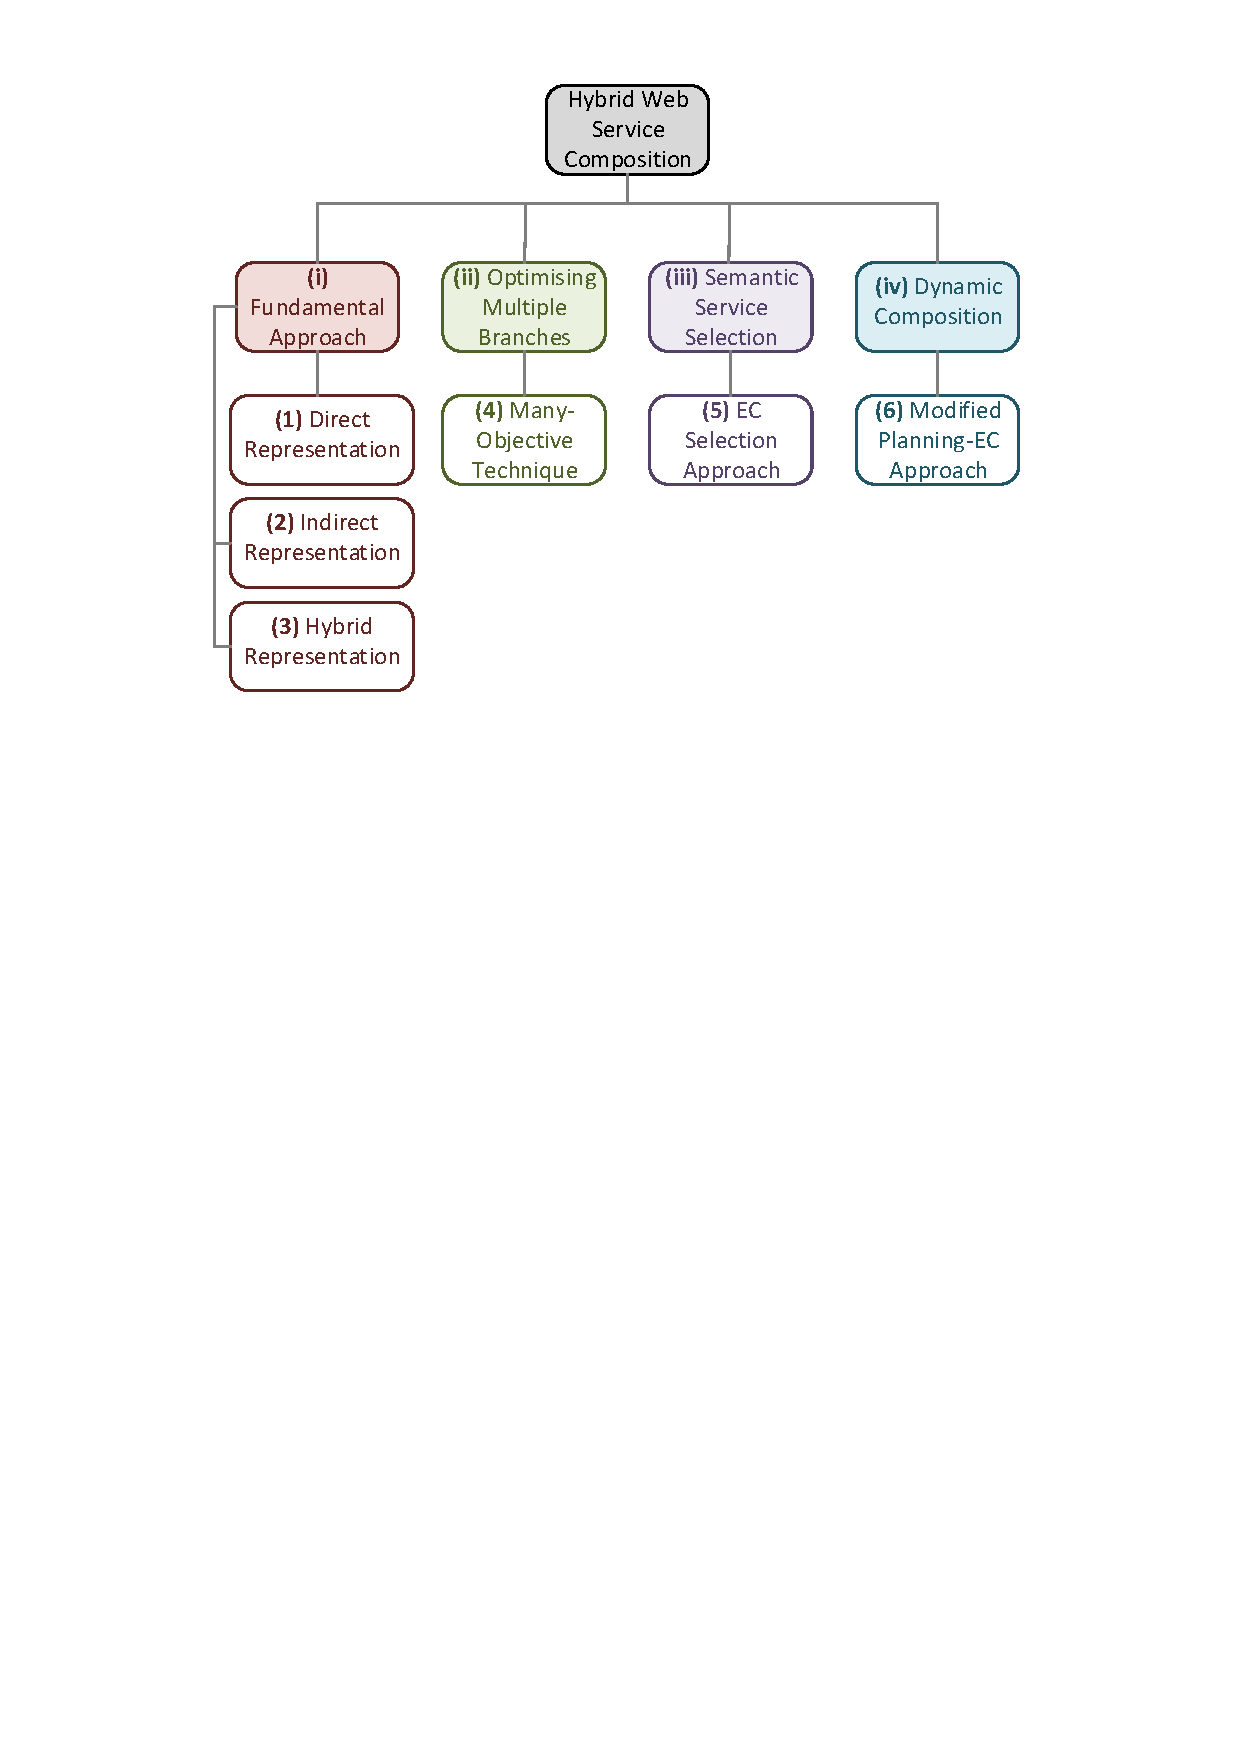
\includegraphics[width=12cm]{objectives.pdf}
}}
\caption{Research objectives and sub-objectives.}
\label{fig:objectives}
\end{figure}

\begin{enumerate}

  \item \label{obj:rep} Create a hybrid QoS-aware Web service composition technique that combines elements of AI planning and evolutionary computation to allow for the optimisation of composition solutions with conditional constraints. One of the key aspects of this technique is the representation of each composition solution. Undoubtedly the simplest model would be that of a linear vector, with each element being a service that should be included into the composition, however this linear structure does not satisfactorily encode the relationships and links between different services. Another problem with a vector is that the EC techniques which use such a representation do not allow for structures of varying lengths, a requirement when performing fully automated composition. The search for a suitable solution representation leads to the following three sub-objectives:
  
  \begin{enumerate}[(a)]
    \item \label{obj:direct} \textit{Propose a direct solution representation for the planning and EC-based Web service composition technique.}\\
    A tree or graph representation is well-suited to represent Web service composition solutions with conditional constraints, since such structures are naturally capable of representing the links between the composing services and multiple execution paths. These structures may be referred to as \textit{direct representations} of solutions, since the genotype and the phenotype of each solution are the same, meaning that solutions are represented directly as they should be interpreted. Proposing a representation based on these structures involves some trade-offs that must be carefully considered, such as the existence of EC techniques that support that structure and the computational cost they incur.
    \item \label{obj:indirect} \textit{Propose an indirect solution representation for the planning and EC-based Web service composition technique.}\\
    Despite the intuitiveness of direct representations, it has been argued in the problem domain of scheduling that indirect representations, where the final result must be decoded from a population candidate, have been shown to have better search performance than their direct counterparts \cite{hart2005evolutionary,craenen2001handle}. Due to this evidence, an indirect candidate representation should be proposed and compared to the direct representation. This indirect representation could be based on the Web service composition Particle Swarm Optimisation (PSO) approach proposed in \cite{da2014graph}.
    \item \label{obj:hybrid} \textit{Propose a hybrid solution representation for the planning and EC-based Web service composition technique.}\\
    In case there is a trade-off between the execution time and the quality of the solutions produced by the direct and indirect representations developed in Objectives \ref{obj:direct} and \ref{obj:indirect}, a hybrid representation should be proposed to combine the strengths of these two approaches. This representation could comprise the structure used in the direct representation with the addition of weights from the indirect representation. Comparisons should be performed to determine whether the hybrid solution presents any performance or quality gains.
  \end{enumerate}
 
 \item \label{obj:mo} Develop a many-objective (MO) approach to optimising the quality of candidate compositions with multiple execution paths, abiding by SLA constraints. Two factors must be taken into account when optimising Web service compositions with multiple execution paths: firstly, each Quality of Service (QoS) attribute must be optimised independently, since they may be conflicting with each other; secondly, each path of the composition must also be independently considered, since the QoS values for each path may vary significantly. The development of this approach can be divided into the following two sub-objectives:
 
   \begin{enumerate}[(a)]
    \item \label{obj:simple-mo} \textit{Propose an unconstrained MO approach for independently optimising the execution paths of a Web service composition solution with conditional constraints.}\\
    The challenge in optimising compositions with multiple execution paths, while at the same time considering several independent quality measures, is the number of dimensions that must be considered simultaneously. On the one hand, encoding each individual quality measure of each execution path as an independent value provides the a very expressive representation of the problem; on the other hand, MO optimisation with a large number of dimensions may result in a solution set that contains many unremarkable solutions. Thus, the proposed approach must handle this issue.
    \item \label{obj:sla-mo} \textit{Extend this MO approach to also consider SLA constraints.}\\
    Once the fundamental MO optimisation approach has been proposed, it should be extended to observe SLA constraints. Note that these constraints must be enforced for each execution path individually, to ensure that all runtime options have been optimised according to the quality parameters of the composition requestor.
   \end{enumerate}
 
 \item \label{obj:semantic} Develop an EC technique for performing semantic Web service selection in the context of a planning-based composition technique. As discussed in Objective \ref{obj:rep}, the composition technique investigated in this thesis combines elements of AI planning and of EC approaches to achieve compositions that are correct, have conditional constraints, and can be optimised according to their QoS attributes. In planning-based approaches to service composition, however, the semantic selection process of candidate atomic services is inefficient, since there are many possible service matches to consider at each planning step. In fact, it may be unfeasible to consider all possible service matches in an exhaustive manner when handling larger service repositories, which invites the use of non-exhaustive approaches such as EC techniques to accomplish this task. Thus, this objective entails the use of an optimisation technique to discover semantically matching services to be included in a composition candidate. Note that this objective aims to investigate the use of an optimisation technique nested within the service selection step of the planning/EC approach.
 
 \item \label{obj:dyna} Modify the planning/EC composition technique to work in a dynamic environment. In a static scenario the planning-EC technique is executed once for a given composition task, returning a composite result under the assumption that the quality levels and the availability of the atomic services included in that result will remain constant. In a more realistic dynamic scenario, however, the quality of the services in the repository may fluctuate and occasionally services may become unavailable. To account for these setbacks, solutions must be corrected and updated in response to changes in the environment. In order to do this, the planning-EC technique is to be modified to retain a population of candidates as alternatives in case of failure, and further generations are to be evolved as the QoS values of services in the repository change, thus leveraging the natural features of Evolutionary Computation. These improvements are to be performed in two steps:
 
 \begin{enumerate}[(a)]
 \item \label{obj:dyna-qos} \textit{Extend planning/EC technique to re-optimise candidates as the quality values of services changes.}\\
 Usually, EC approaches dedicated to Web service composition create a population of candidates, optimise this population, and identify the best solution candidate, discarding the others in the process. In a dynamic scenario, disposing of the remaining candidates would be wasteful, since some of these alternative solutions may become promising as quality values change. Instead of destroying the population, the extended technique should maintain it for future re-optimisation. A key challenge in this approach is striking a balance between population diversity and effective optimisation.
 \item \label{obj:dyna-fail} \textit{Create a strategy for handling service failure using other candidates in the population.}\\
 In addition to quality changes, the atomic services used in a composition may occasionally fail/become unavailable. An alternative execution plan must be used to prevent the composite service from being impacted, and the proposed solution is to select as efficiently as possible an unaffected candidate from the population as the replacement.
 \end{enumerate}
 
\end{enumerate}

\section{Published Papers}

During the initial stage of this research, some investigation was carried out on the suitability of different candidate representations for EC-based Web service composition. This culminated in the publication of the following papers:

\begin{itemize}
 \item Alexandre Sawczuk Da Silva, Hui Ma and Mengjie Zhang. "A GP Approach to QoS-Aware Web Service Composition and Selection". \textit{Proceedings of the 10th International Conference on Simulated Evolution and Learning (SEAL 2014). Lecture Notes in Computer Science}. \textbf{Vol. 8886}. Dunedin, New Zealand. December 15-18, 2014. pp. 180-191.
 \item Alexandre Sawczuk da Silva, Hui Ma and Mengjie Zhang. "A GP Approach to QoS-Aware Web Service Composition including Conditional Constraints". \textit{Proceedings of 2015 IEEE Congress on Evolutionary Computation (CEC 2015)}. Sendai, Japan. 25-28 May, 2015 (To Appear)
 \item Alexandre Sawczuk da Silva, Hui Ma and Mengjie Zhang. "GraphEvol: A Graph Evolution Technique for Web Service Composition". \textit{Proceedings of the 26th International Conference on Database and Expert System Applications (DEXA 2015)}. Valencia, Spain. 1-4 September, 2015 (Accepted)
\end{itemize}


\section{Organisation of Proposal}
The remainder of the proposal is organised as follows: Chapter \ref{C:review} provides a fundamental definition of the Web service composition problem and performs a literature review covering a range of works in this field; Chapter \ref{C:preliminary} discusses the preliminary work carried out to explore the hybridisation of AI planning techniques and EC-based techniques for Web service composition, one of the key ideas proposed in this project; Chapter \ref{C:plan} presents a plan detailing this project's intended contributions, a project timeline, and a thesis outline.
